%
% Шаблон для ВКР бакалавра 2023
%

\documentclass[a4paper,12pt]{article}
\usepackage{vkriate}

% Настройки для окружений с подчеркиваниями для подписей и пр.
\setFRMfontencoding{T2A}
\setFRMdfontencoding{T2A}
% thanks to A.Starikov
\setFRMfontfamily{cmr}
\setFRMdfontfamily{ptm}
\setFRMdfontsize{10pt}

% задает длину поля для подписи на титульной странице
\newFRMfield{xtitlesign}{32mm}

% поле для факультета или кафедры
\newFRMfield{fcath}{65mm}

%имя файла с библиографией в формате BibTex
\addbibresource{rbiblio.bib}

\begin{document}

% счетчики страниц, рисунков, таблиц
\regtotcounter{page}
\regtotcounter{figure}
\regtotcounter{table}

\renewcommand{\refname}{\centerline{СПИСОК ИСПОЛЬЗОВАННЫХ ИСТОЧНИКОВ}} 
\renewcommand{\contentsname}{\centerline{СОДЕРЖАНИЕ}} 
%\renewcommand{\refname}{Список источников}  % По умолчанию "Список литературы" (article)
%\renewcommand{\bibname}{Литература}  % По умолчанию "Литература" (book и report)

% титульная страница
\thispagestyle{empty}
\begin{center} \small
\textbf{МИНИСТЕРСТВО НАУКИ И ВЫСШЕГО ОБРАЗОВАНИЯ\\ РОССИЙСКОЙ ФЕДЕРАЦИИ}\\
ФЕДЕРАЛЬНОЕ ГОСУДАРСТВЕННОЕ АВТОНОМНОЕ ОБРАЗОВАТЕЛЬНОЕ УЧРЕЖДЕНИЕ
ВЫСШЕГО  ОБРАЗОВАНИЯ\\
«Национальный исследовательский ядерный университет «МИФИ»\\
\textbf{Обнинский институт атомной энергетики} – \\
филиал федерального государственного автономного образовательного учреждения высшего\\
образования «Национальный исследовательский ядерный университет «МИФИ»\\
(ИАТЭ НИЯУ МИФИ)
\end{center}
%\vfill
\medskip

% Направление подготовки следует уточнять,
% магистры и бакалавры могут иметь разные наименования
\begin{center}
\begin{tabular}{rl}
Отделение & \useFRMfield{fcath}[\large Интеллектуальные кибернетические системы] \\ 
%Направление подготовки & \useFRMfield{fcath}[\large Информационные системы и технологии] \\ 
\end{tabular} 
\end{center}

\vfill

\large 

\begin{center}
\textbf{\Large Выпускная квалификационная работа --- } \\
\textbf{\Large бакалаврская работа}\\
	
	\medskip

{ \normalsize
по направлению подготовки  \textbf{09.03.02 Информационные  системы и технологии}\\

Направленность (профиль) \textbf{Информационные технологии}
}	
\vfill
\vfill
\medskip

\textbf{\Large 
		<<Разработка приложения для автоматизированного статистического анализа данных, полученных при проведении КГО стендовым методом на реакторах типа ВВЭР>>
	}
	
\end{center}

\vspace{1cm}

\begin{center}
\begin{tabular*}{\textwidth}{p{78mm}p{33mm}p{64mm}}
	Выполнил:\\студент гр. ИС2-Б20 & \useFRMfield{xtitlesign} & Костевич А.Е.\\
	& & \\
% должность, научная степень руководителя
	Руководитель ВКР,\\старший преподаватель ОИКС & \useFRMfield{xtitlesign} & Радаев А.В. \\
	& & \\
	
	Нормоконтроль\\ доцент отделения ИКС, к.ф.-м.н. & \useFRMfield{xtitlesign} &  Качанов~Б.В. \\
	& & \\
	% Если нужно добавить консультанта - раскомментируйте две строчки ниже
	%Консультант ВКР бакалавра\\организация, должность, звание  & \useFRMfield{xtitlesign} & К.О.Нсультант\\
	%& & \\
%	Рецензент\\к.ф.-м.н.,   & \useFRMfield{xtitlesign} & В.А. Чепурко\\
	
	& & \\
	Выпускная квалификационная \\ работа допущена к защите & \useFRMfield{xtitlesign} &  \\
	& & \\
	Руководитель\\ образовательной программы \\
	09.03.02 Информационные системы и технологии\\
	канд. тех. наук  & \useFRMfield{xtitlesign} &Мирзеабасов~О.А. \\
	
\end{tabular*}
\end{center}

\vfill
\large

\begin{center}
Обнинск, 2024 г
\end{center}

\onehalfspacing

\pagebreak

% реферат
\thispagestyle{empty}

\section*{\centering РЕФЕРАТ}

\thispagestyle{empty} % страница реферата не нумеруется

%Объектом разработки является мобильное приложения для визуализации погодных явлений в дополненной реальности для устройств под управлением ОС Android.
%Целью работы является создание мобильного приложения для визуализации погодных явлений в дополненной реальности.
%Задачами ВКР являются выбор и освоение инструментов для создания образцов дополненной реальности, создание трехмерных моделей для визуализации, разработка алгоритма для объединения моделей в единые сцены, создание пользовательского интерфейса для навигации и выбора сцен с явлениями, добавление описания к явлениям и возможность вывода его на экран устройства, добавление возможности изменения характеристик явлений.
%Новизна работы заключается в создании приложения, которое объединяет в себе возможность визуализации явлений, с использованием средств дополненной реальности, текстового описания, включающего в себя уровень опасности и возможные последствия, и возможность изменения характеристик явлений.
%Ключевые слова: дополненная реальность, мобильное приложение, гидрометеорологические явления, Unity, Android, повышение информирования.

Работа \total{page} стр., \total{table} табл., \total{figure} рис., \totalmycitecounts ист. 

РАЗРАБОТКА ПРИЛОЖЕНИЯ ДЛЯ АВТОМАТИЗИРОВАННОГО СТАТИСТИЧЕСКОГО АНАЛИЗА ДАННЫХ, ПОЛУЧЕННЫХ ПРИ ПРОВЕДЕНИИ КГО СТЕНДОВЫМ МЕТОДОМ ДЛЯ РЕАКТОРОВ ТИПА ВВЭР.

Объектом разработки является настольное приложение с графическим интерфейсом, поддерживающее функции визуализации, экспорта, а также статистического анализа данных.

Целью данной работы является разработка программного обеспечения для повышения точности и упрощения процесса анализа данных, полученных при проведении КГО в пеналах СОДС. 

Задачами ВКР являются изучение и анализ метода проведения КГО, выбор критериев для анализа данных, выбор и освоение инструментов разработки, реализация алгоритмов анализа данных, а также разработка приложения.

В работе производится подробный анализ существующего подхода к проведению процедуры и анализу данных КГО на реакторах типа ВВЭР, приводятся предложения по улучшению и автоматизации этого подхода, а также описывается процесс разработки программного обеспечения с учётом внесённых предложений. Разработанное приложение было успешно апробировано на Нововоронежской АЭС.

\pagebreak
\thispagestyle{empty}

\section*{\centering ОПРЕДЕЛЕНИЯ}

\thispagestyle{empty} % страница определений не нумеруется

Реперный радионуклид --- радионуклид, по выходу которого из твэла в
теплоноситель первого контура судят о герметичности оболочки твэла, так как
он обладает ядерно-физическими и химическими характеристиками,
позволяющими надежно регистрировать его в условиях эксперимента.

Негерметичный твэл - твэл, в оболочке которого имеется повреждение,
приводящее к выходу продуктов деления из него.

Негерметичная ТВС --- ТВС, в составе которой имеются негерметичные твэлы.

\pagebreak

\section*{\centering ОБОЗНАЧЕНИЯ И СОКРАЩЕНИЯ}

\thispagestyle{empty} % страница обозначений и сокращений не нумеруется

БВ --- Бассейн выдержки.

ВВЭР --- Водо-водяной энергетический реактор.

КГО --- Контроль герметичности оболочек.

ЛПР --- Лицо, принимающее решение.

ПД --- Продукты деления.

ПК --- Продукты коррозии.

СОДС --- Система обнаружения дефектных сборок.

ТВС --- Тепловыделяющая сборка.

\pagebreak

% титульная страница - номер 1, остальные страницы до Содержания не нумеруются
\tocloftpagestyle{empty}

\tableofcontents
% если нужно добавить "Стр." над номерами страниц - раскомментируйте следующую команду
%\addtocontents{toc}{~\hfill\textbf{Стр.}\par}

\thispagestyle{empty}

\pagebreak

\setcounter{page}{3}

\section*{\centering ВВЕДЕНИЕ}
\addcontentsline{toc}{section}{ВВЕДЕНИЕ}
% пример введения

Атомные электростанции играют ключевую роль в современной
энергетике. Однако сопутствующие ядерной энергетике риски требуют
непрерывного совершенствования методов контроля и обслуживания ядерных установок.

В частности, одним из значимых аспектов эксплуатации ядерных реакторов является контроль герметичности оболочек тепловыделяющих
элементов. В настоящее время анализ данных, полученных при проведении
КГО, частично осуществляется в ручном режиме, что требует значительных ресурсов времени и труда. Более того, этот подход подвержен человеческим ошибкам и может ограничивать возможности в проведении анализа данных с высокой точностью и скоростью.

Как известно, одним из недостатков реактора типа ВВЭР является
невозможность перегрузки топлива без остановки реактора и ошибка,
допущенная при принятии решения относительно герметичности ТВС, может
потребовать незапланированную остановку реактора, что влечёт за собой
существенные экономические издержки.

Цель настоящей работы заключается в разработке программного обеспечения, работа которого направлена на повышение эффективности
и достоверности результатов КГО, а также снижение трудовых затрат.

В данной работе будет проведен обзор существующего метода обработки результатов КГО, приведены предложения по его автоматизации, а также описан процесс создания прототипа программного обеспечения.
%\cite{SoetaertRJ2010}.
%\cite{kotelnikov}  % текст введения в файле intro.tex
\pagebreak

%\input{Post_zad}
\pagebreak
% первая часть

\section{Глава 1 Обзор существующей методики проведения процедуры КГО стендовым методом}

\subsection{Основные положения}

В данной работе рассматривается метод КГО в пеналах СОДС, который является одним из наиболее надёжных
способов определения негерметичных ТВС. СОДС входит в состав обязательного оборудования всех действующих и проектируемых АЭС с реактором ВВЭР.

Метод основан на измерении утечки ПД из-под оболочек твэлов путем гамма-спектрометрического анализа изотопного состава проб воды, отбираемых из контура циркуляции СОДС, по активности реперных радионуклидов $^{131}$I, $^{134}$Cs, $^{136}$Cs, $^{137}$Cs и $^{133}$Xe. Инициирование выхода радионуклидов в воду стенда КГО осуществляется посредством изменения давления циркулирующей по контуру стенда воды в процессе выдержки ТВС в этой воде -- настаивании.


\subsection{Процедура проведения КГО стендовым методом}
1. Процедура проведения КГО начинается проведения испытаний для каждой ТВС в пеналах СОДС с последующим отбором проб воды. 

Проверка ТВС проводится при циркуляции воды по контуру стенда КГО без ее замены и состоит из двух циклов:

- Настаивание ТВС при изыбыточном (верхнем) давлении в контуре от 4,5 * 10$^{5}$ Па до 6,0 * 10$^{5}$ Па продолжительностью 5 минут.

- Настаивание ТВС при избыточном (нижнем) давлении в контуре от 1,0 * 10$^{5}$ Па до 1,5 * 10$^{5}$ Па до полного перемешивания (не менее 15 минут).

С целью соблюдения одинаковых условий испытаний требуется, чтобы значения верхнего и нижнего избыточного давления были одинаковыми при проверке всех ТВС. 

2. После завершения настаивания ТВС производится отбор пробы воды из контура стенда КГО.

3. В каждой $j$-ой пробе воды, взятой из стенда КГО при испытании $j$-ой ТВС, на спектрометрической установке измеряются значения удельной активности и приводятся на момент останова реактора:

- $A_{j,кго}^{i}$ --- реперных $i$-х радионуклидов продуктов деления ($^{131}$I, $^{134}$Cs, $^{136}$Cs, $^{137}$Cs и $^{133}$Xe)

- $A_{j,кго}^{i'}$ --- радионуклида продукта коррозии ($^{54}$Mn или $^{58}$Co, $^{60}$Co, $^{51}$Cr, $^{59}$Fe).

4. Для учета фоновой активности радионуклидов йода, цезия и
продуктов коррозии периодически производится измерение их активности
в воде, подаваемой в стенд КГО (с каждой вновь приготовленной порцией
раствора борной кислоты на СВО), и в бассейне выдержки (один раз в
сутки).

5. Проверка фоновой составляющей за счет загрязнения стенда
радиоактивными продуктами (холостая проба) производится перед началом
работ по КГО, а также периодически (не реже одного раза в сутки). Для этого
без загрузки ТВС в пенал проводятся все операции по промывке контура и
настаиванию с отбором и анализом пробы.

6. Итогом проведения спектрометрического анализа проб воды является
таблица значений, в которых для каждой $j$-ой ТВС приводятся в соответствие
значения активности $A_{j,кго}^{i}$ каждого из регистрируемых реперных радионуклидов
и $A_{j,кго}^{i'}$ продуктов коррозии. Статистический анализ результатов
измерения проводится для ТВС, в пробах которых значимо регистрировались
ПД. Результаты измерений ТВС, при проверке которых реперные ПД не
регистрировались, из статистического расчета исключаются.

\subsection{Обработка результатов}
1. Анализ герметичности ТВС основан на выборочном поиске выбросов методом "3 сигм". Зачастую данный метод наиболее показателен в выборках, извлечённых из нормально распределённой генеральной совокупности. Однако этот метод(так же как и обратный ему "Z оценка") устойчив и для других видов распределения.

2. Процедура КГО, описанная в параграфе 1.2, с учётом времени и объёма испытаний может проходить до нескольких недель. Кроме того, с течением времени может изменяться концентрация борной кислоты в БВ и в воде, подаваемой на стенд КГО. В связи с этим значения активностей ПД, полученные в разное время, могут принадлежать разным статистическим распределениям.

3. Исходя из изложенного в 1.3.1-1.3.2 требуется разделять исходные данные на выборки, принадлежащие одному статистическому распределению. Поиск негерметичных ТВС происходит в каждой выборке раздельно. 

\subsection{Формулы}

Формулы в \LaTeXe\ выглядят достаточно красиво, как строчные --- $E=mc^2$, так и выключные (см. \ref{eq:pi}):

\begin{equation} \label{eq:pi}
\pi = \int\limits_0^1 \frac{4}{1+x^2} dx
\end{equation}  % первая глава - в файле part1.tex
\pagebreak
% вторая часть
\section{Предложения по улучшению методики обработки данных}

\subsection{Проблемы существующего подхода}
Рассмотрев методику проведения процедуры КГО согласно\cite{RD} можно выделить несколько замечаний, которые можно пересмотреть:

1. Метод анализа данных, приведённый в параграфе 1.3, основывается на поиске выбросов по правилу "3 сигм". Данное правило утверждает, что  абсолютная величина отклонения нормально распределённой случайной величины от её математического ожидания не превосходит трёх среднеквадратичных отклонений с вероятностью\cite{KremerMatstat}:
\begin{equation} \label{eq:3sigma_rule}
	P(|X - m| < 3\sigma)  = 0,9973
\end{equation}

Проблема этого метода заключается в том, что он применим для выборок, значения которых извлечены из нормально распределённых генеральных совокупностей. Но в случае проведения КГО(согласно разделу 1) нет достаточных оснований утверждать, что все значения активностей будут распределены по нормальному закону. Следовательно, требуется проверить характер распределения для каждой выборки с целью установления корректности применения метода "3 сигм".

Кроме того, среднее и среднеквадратическое отклонение, рассчитываемые в данном методе, также изменяются под воздействием аномальных значений, что приводит к маскировке выбросов\cite{emissions}. Следовательно, имеет смысл рассмотреть альтернативы, например метод межквартильного размаха(IQR).

2. Процедура КГО с учётом времени и объёма испытаний может проходить до нескольких недель. С течением времени в БВ, а также в воде, подаваемой на стенд КГО, может изменяться концентрация борной кислоты с целью борного регулирования, что негативно сказывается на однородности условий проведения испытаний. В связи с этим значения активностей ПД, полученные в разное время, могут принадлежать разным статистическим распределениям, следовательно, анализироваться должны отдельно. 

Согласно пункту 1.3.3, разделение на выборки происходит "На основании визуального анализа"\ графических данных. Хочу отметить, что в изучаемой методике существует способ анализа полученных выборок на принадлежность к одному статистическому распределению с целью объединения нескольких выборок, но он не учитывает анализ на корректность разбиения исходных данных. В связи с вышеперечисленным возникает необходимость проверки данных в выборках, полученных на основании визуального анализа.

3. Описанный процесс анализа данных производится в ручном режиме с использованием программного комплекса Excel. Автоматизация этого процесса позволит снизить вероятность ошибок, ведущих к преждевременной остановке реактора, а также снизить потребность во временных и трудовых затратах.

\subsection{Предложения по улучшению}

\subsubsection{Метод IQR}

Учитывая изложенное в 2.1.1, в качестве альтернативы методу "3 сигм"\ имеет смысл рассмотреть метод поиска выбросов с помощью межквартильного размаха(Interquartile range/IQR).

Межквартильный размах (IQR) — это статистическая мера, равная разности между первым и третьим квартилями распределения (25-м и 75-м процентилями). Первый квартиль (Q1) — это значение, ниже которого находится 25\% данных, а третий квартиль (Q3) — это значение, ниже которого находится 75\% данных. Можно так же сказать, что интерквартильный размах это половина выборки, центрированная относительно медианы. 

Этот показатель полезен для оценки изменчивости признака в асимметричных распределениях или наборах данных с выбросами. Интерквартильный размах является устойчивым(робастным) аналогом дисперсии, поскольку не подвержен влиянию аномальных значений. Именно поэтому он является наиболее перспективным аналогом методу "3 сигм". 
Таким образом, интерквартильный размах позволяет обнаруживать аномальные значения, являясь альтернативой среднеквадратическому отклонению, которое эффективно только для нормально распределенных данных. IQR — это непараметрическая оценка, что делает его применимым для анализа данных любого распределения.

В современных практиках поиска выбросов с использованием межквартильного размаха применяется следующий метод расчёта критических значений:
\begin{equation} \label{eq:IQRmin}
	X^{min}  = Q1-1.5*IQR
\end{equation}

\begin{equation} \label{eq:IQRmax}
	X^{max}  = Q3+1.5*IQR
\end{equation}


На рисунке~\ref{fig:ris6} приведена иллюстрация коэффициента IQR для нормального распределения.

\begin{figure}[H]
	\centering
	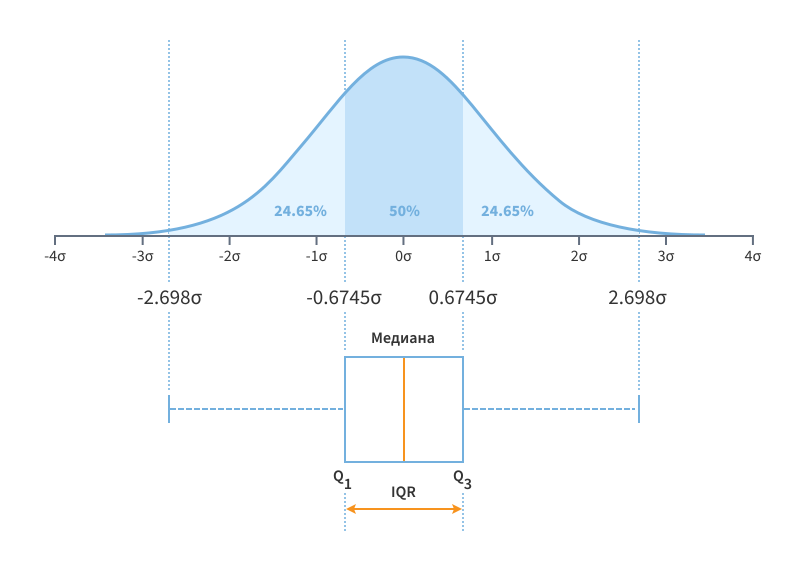
\includegraphics[width=1\linewidth]{pics/ris6} % изображения хранятся в подкаталоге pics
	\caption{Графическое представление межквартильного размаха на примере нормального распределения.}
	\label{fig:ris6} % эта метка позволяет ссылаться на рисунок в тексте
\end{figure}

Из рисунка~\ref{fig:ris6} видно, что данный подход в случае нормального распределения охватывает интервал:
\begin{equation} \label{eq:IQRP}
	P(|X^{min/max} - X| < 2.698\sigma)  = 0,9545
\end{equation}

%Использование этого метода в качестве альтернативы методу "3 сигм"\ с точностью, требуемой в условии \ref{eq:3sigma_rule}, требует замену коэффициента при IQR в формулах~\ref{eq:IQRmin}-\ref{eq:IQRmax}.

%\begin{equation} \label{eq:IQR}
%	P(Q3+1.7*IQR - X < 3\sigma)  = 0,9973
%\end{equation}

\subsubsection{U-критерий Манна-Уитни}

\subsubsection{Критерий Шапиро-Уилка}

\subsubsection{Критерий Стьюдента для независимых выборок}


% 3. Исходя из изложенного в 1.3.1-1.3.2 требуется разделять исходные данные на выборки, принадлежащие как минимум одному статистическому распределению, в идеальном случае требуется, чтобы выборка подчинялась нормальному закону распределения. % вторая глава - в файле part2.tex
\pagebreak
% вторая часть

\section{Проектирование приложения с учётом внесённых предложений}

\subsection{Требования к проектируемому приложению}\label{trebovaniya}

С целью обеспечения наибольшей точности и минимизации рисков,
связанных с возможностью некорректного принятия решений относительно
герметичности ТВС, предлагаю разработать приложение для обработки и анализа данных, полученных при КГО стендовым водным методом на реакторе типа ВВЭР, которое призвано помочь лицу, принимающему решения относительно
герметичности ТВС. Основной задачей данного приложения является автоматизированная(под контролем ЛПР) обработка и анализ данных. Исходные данные хранятся в табличном виде в формате ODS. Под обработкой и анализом данных понимается разделение исходных данных на выборки, принадлежащие к
одному статистическому распределению, произведение всех необходимых
расчётов, а также принятие решения относительно герметичности ТВС. После предварительного анализа методики, описанной в главе 1, а также учитывая изложенное в главе 2, могу выдвинуть следующие требования к приложению:

1. Приложение должно наглядно демонстрировать ЛПР основания принятия
решения относительно герметичности ТВС, т.е. иметь обширный функционал
для визуализации и экспорта графиков распределений, негерметичных ТВС и т.д. Исходя из этого был выбран формат настольного приложения с графическим интерфейсом.

2. Приложение должно иметь функционал для проведения статистических тестов с целью проверки выборок, заданных пользователем, на принадлежность одному статистическому распределению, а также на характер распределения.

В качестве статистических тестов предлагаю использовать:
\begin{itemize}
	\item U-критерий Манна-Уитни --- c целью установления принадлежности выборок к одному статистическому распределению
	\item Критерий Шапиро-Уилка~\cite{RANstat} --- с целью проверки на отклонение распределения выборки от нормального закона.
	\item Критерий Стьюдента для независимых выборок~--- c целью установления статистически значимых различий между независимыми выборками, независимые выборки должны быть распределены нормально (Проверяется критерием Шапиро-Уилка).
\end{itemize}

3. Приложение должно поддерживать поиск выбросов методами "IQR"\ и "3 cигма". По усмотрению ЛПР может применяться любой метод в зависимости от ситуации.

4. Приложение должно иметь возможности для экспорта всех преобразованных
данных, на основании которых принимались решения о герметичности, в
исходный ODS формат.

\subsection{Обзор инструментов разработки}

Для разработки приложения на основании требований, описанных в \ref{trebovaniya}, были выбраны следующие инструменты:

1. Язык программирования Python - высокоуровневый, интерпретируемый, объектно-ориентированный язык программирования, который широко используется для разработки веб-приложений, научных вычислений, анализа данных, искусственного интеллекта, автоматизации задач и многих других областей. В совокупности с большим набором пользовательских библиотек, python предоставляет мощные инструменты для обработки, анализа и визуализации данных. 

В качестве альтернативы Python рассматривался язык R. R предоставляет более широкий спектр функций по обработке и анализу данных, но набор инструментов для визуализации, а также создания интерфейса приложений ограничен. Именно этот фактор стал решающим в пользу Python.

2. Библиотека Pandas -  программная библиотека на языке Python для обработки и анализа данных. Работа Pandas с данными строится поверх библиотеки NumPy, являющейся инструментом более низкого уровня. Предоставляет специальные структуры данных и операции для манипулирования табличными данными. Преимущество Pandas заключается в дешевизне операций и скорости работы, что делает ее неотъемлемым инструментом для анализа данных, машинного обучения, статистики и других областей, где требуется работа с табличными данными.

3. Библиотека NumPy предоставляет эффективные контейнеры для
работы с массивами и матрицами данных. В совокупности с Pandas она широко используется для выполнения математических операций и вычислений в Python.

4. SciPy --- библиотека, основанная на расширении NumPy, которая применяется для более сложных научных и инженерных вычислений. SciPy в основном написана на Python и частично на языках C, C++ и Fortran, в связи с чем отличается высокой производительностью и скоростью работы. В рамках разработки приложения использовался модуль scipy.stats, который предоставляет обширный функционал для проведения статистических вычислений.

5. Библиотеки Matplotlib и Seaborn. Эти библиотеки предоставляют
возможности для визуализации данных в Python. Matplotlib является основной
библиотекой для создания различных типов графиков, в то время как Seaborn
предоставляет более высокоуровневый интерфейс для создания
статистических графиков.

6. PyQt --- набор расширений кроссплатформенного графического фреймворка Qt, выполненный в виде библиотеки Python. Qt --- фреймворк для разработки кроссплатформенного программного обеспечения c графическим интерфейсом, написанный на языке программирования C++.

\subsection{Архитектура приложения}

\subsection{Пользовательский сценарий использования}

Ниже приведены шаги, которые будет выполнять пользователь при работе с проектируемым приложением:

1. Импорт данных: пользователь выбирает файл в формате .ods с входными данными для анализа.

2. Анализ входных данных: перед пользователем открывается окно, в котором имеется возможность построения и гибкого редактирования графиков по входным данным. Согласно, 1.3.3 на основании визуального анализа графиков, пользователь разделяет входные данные на выборки.

3. Анализ выборок: После разбиения входных данных возникает возможность выполнения статистических тестов для каждой выборки. Пользователь выбирает выборку и анализируемую величину, после чего запускает статистические тесты. Результаты тестов выводятся в отдельном окне для каждой выборки и анализируемой величины. На основании результатов тестов, пользователь делает заключение о корректности разбиения входных данных и возможности дальнейшего анализа.

В случае, если результаты статистических тестов не позволяют проводить дальнейший поиск выбросов в выборках, окно с выборками закрывается и шаги 2-3 повторяются до тех пор, пока все выборки не будут удовлетворять условиям, позволяющим проводить поиск выбросов.

4.  % третья глава - в файле part3.tex
\pagebreak
% вторая часть

\section{Разработка приложения}

\subsection{Исходный код}

Исходный код программ можно добавить с помощью окружений, определенных сразу после преамбулы. Пример --- на листинге~\ref{lst:1}.


\begin{flushleft}
\needspace{3\baselineskip}
\captionof{Program}{Пример кода на языке R} \label{lst:1}
\begin{MyCodes}
# Проверка и тестирование пакета deSolve
require(deSolve)
require(rgl)

# система Хиндмарша - Розе с параметрами
# используются параметры в виде списка (parms$a etc)
hindrose <- function(t,y,parms)
{
 ydot <- vector(len=3)
 ydot[1] <- y[2] - parms$a * y[1]^3 + parms$b*y[1]^2 + parms$Iext - y[3]
 ydot[2] <- parms$c - parms$d*y[1]^2 - y[2]
 ydot[3] <- parms$r * (parms$s*(y[1]-parms$xs)-y[3])
 return(list(ydot))
}
\end{MyCodes}
\end{flushleft} % четвёртая глава - в файле part4.tex
\pagebreak

% если есть еще разделы - сохраните их в соответствующих файлах и раскомментируйте строки ниже, при необходимости добавьте еще
%% вторая часть

\section{Проектирование приложения с учётом внесённых предложений}

\subsection{Требования к проектируемому приложению}\label{trebovaniya}

С целью обеспечения наибольшей точности и минимизации рисков,
связанных с возможностью некорректного принятия решений относительно
герметичности ТВС, предлагаю разработать приложение для обработки и анализа данных, полученных при КГО стендовым водным методом на реакторе типа ВВЭР, которое призвано помочь лицу, принимающему решения относительно
герметичности ТВС. Основной задачей данного приложения является автоматизированная(под контролем ЛПР) обработка и анализ данных. Исходные данные хранятся в табличном виде в формате ODS. Под обработкой и анализом данных понимается разделение исходных данных на выборки, принадлежащие к
одному статистическому распределению, произведение всех необходимых
расчётов, а также принятие решения относительно герметичности ТВС. После предварительного анализа методики, описанной в главе 1, а также учитывая изложенное в главе 2, могу выдвинуть следующие требования к приложению:

1. Приложение должно наглядно демонстрировать ЛПР основания принятия
решения относительно герметичности ТВС, т.е. иметь обширный функционал
для визуализации и экспорта графиков распределений, негерметичных ТВС и т.д. Исходя из этого был выбран формат настольного приложения с графическим интерфейсом.

2. Приложение должно иметь функционал для проведения статистических тестов с целью проверки выборок, заданных пользователем, на принадлежность одному статистическому распределению, а также на характер распределения.

В качестве статистических тестов предлагаю использовать:
\begin{itemize}
	\item U-критерий Манна-Уитни --- c целью установления принадлежности выборок к одному статистическому распределению
	\item Критерий Шапиро-Уилка~\cite{RANstat} --- с целью проверки на отклонение распределения выборки от нормального закона.
	\item Критерий Стьюдента для независимых выборок~--- c целью установления статистически значимых различий между независимыми выборками, независимые выборки должны быть распределены нормально (Проверяется критерием Шапиро-Уилка).
\end{itemize}

3. Приложение должно поддерживать поиск выбросов методами "IQR"\ и "3 cигма". По усмотрению ЛПР может применяться любой метод в зависимости от ситуации.

4. Приложение должно иметь возможности для экспорта всех преобразованных
данных, на основании которых принимались решения о герметичности, в
исходный ODS формат.

\subsection{Обзор инструментов разработки}

Для разработки приложения на основании требований, описанных в \ref{trebovaniya}, были выбраны следующие инструменты:

1. Язык программирования Python - высокоуровневый, интерпретируемый, объектно-ориентированный язык программирования, который широко используется для разработки веб-приложений, научных вычислений, анализа данных, искусственного интеллекта, автоматизации задач и многих других областей. В совокупности с большим набором пользовательских библиотек, python предоставляет мощные инструменты для обработки, анализа и визуализации данных. 

В качестве альтернативы Python рассматривался язык R. R предоставляет более широкий спектр функций по обработке и анализу данных, но набор инструментов для визуализации, а также создания интерфейса приложений ограничен. Именно этот фактор стал решающим в пользу Python.

2. Библиотека Pandas -  программная библиотека на языке Python для обработки и анализа данных. Работа Pandas с данными строится поверх библиотеки NumPy, являющейся инструментом более низкого уровня. Предоставляет специальные структуры данных и операции для манипулирования табличными данными. Преимущество Pandas заключается в дешевизне операций и скорости работы, что делает ее неотъемлемым инструментом для анализа данных, машинного обучения, статистики и других областей, где требуется работа с табличными данными.

3. Библиотека NumPy предоставляет эффективные контейнеры для
работы с массивами и матрицами данных. В совокупности с Pandas она широко используется для выполнения математических операций и вычислений в Python.

4. SciPy --- библиотека, основанная на расширении NumPy, которая применяется для более сложных научных и инженерных вычислений. SciPy в основном написана на Python и частично на языках C, C++ и Fortran, в связи с чем отличается высокой производительностью и скоростью работы. В рамках разработки приложения использовался модуль scipy.stats, который предоставляет обширный функционал для проведения статистических вычислений.

5. Библиотеки Matplotlib и Seaborn. Эти библиотеки предоставляют
возможности для визуализации данных в Python. Matplotlib является основной
библиотекой для создания различных типов графиков, в то время как Seaborn
предоставляет более высокоуровневый интерфейс для создания
статистических графиков.

6. PyQt --- набор расширений кроссплатформенного графического фреймворка Qt, выполненный в виде библиотеки Python. Qt --- фреймворк для разработки кроссплатформенного программного обеспечения c графическим интерфейсом, написанный на языке программирования C++.

\subsection{Архитектура приложения}

\subsection{Пользовательский сценарий использования}

Ниже приведены шаги, которые будет выполнять пользователь при работе с проектируемым приложением:

1. Импорт данных: пользователь выбирает файл в формате .ods с входными данными для анализа.

2. Анализ входных данных: перед пользователем открывается окно, в котором имеется возможность построения и гибкого редактирования графиков по входным данным. Согласно, 1.3.3 на основании визуального анализа графиков, пользователь разделяет входные данные на выборки.

3. Анализ выборок: После разбиения входных данных возникает возможность выполнения статистических тестов для каждой выборки. Пользователь выбирает выборку и анализируемую величину, после чего запускает статистические тесты. Результаты тестов выводятся в отдельном окне для каждой выборки и анализируемой величины. На основании результатов тестов, пользователь делает заключение о корректности разбиения входных данных и возможности дальнейшего анализа.

В случае, если результаты статистических тестов не позволяют проводить дальнейший поиск выбросов в выборках, окно с выборками закрывается и шаги 2-3 повторяются до тех пор, пока все выборки не будут удовлетворять условиям, позволяющим проводить поиск выбросов.

4.   % третья глава - в файле part3.tex
%\pagebreak

%% вторая часть

\section{Разработка приложения}

\subsection{Исходный код}

Исходный код программ можно добавить с помощью окружений, определенных сразу после преамбулы. Пример --- на листинге~\ref{lst:1}.


\begin{flushleft}
\needspace{3\baselineskip}
\captionof{Program}{Пример кода на языке R} \label{lst:1}
\begin{MyCodes}
# Проверка и тестирование пакета deSolve
require(deSolve)
require(rgl)

# система Хиндмарша - Розе с параметрами
# используются параметры в виде списка (parms$a etc)
hindrose <- function(t,y,parms)
{
 ydot <- vector(len=3)
 ydot[1] <- y[2] - parms$a * y[1]^3 + parms$b*y[1]^2 + parms$Iext - y[3]
 ydot[2] <- parms$c - parms$d*y[1]^2 - y[2]
 ydot[3] <- parms$r * (parms$s*(y[1]-parms$xs)-y[3])
 return(list(ydot))
}
\end{MyCodes}
\end{flushleft} % четвертая глава - в файле part4.tex
%\pagebreak

%\input{part5}  % пятая глава - в файле part5.tex
%\pagebreak

\section*{\centering ЗАКЛЮЧЕНИЕ}
\addcontentsline{toc}{section}{ЗАКЛЮЧЕНИЕ}

В ходе проделанной работы был проведён анализ существующего метода анализа данных КГО в пеналах СОДС на реакторах ВВЭР типа. Были приведены предложения по улучшению и автоматизации данного процесса. Было реализовано программное обеспечение с учётом внесённых предложений, в которой реализованы следующие функции:

\begin{itemize}
\item Поиск выбросов методом "3 сигм".
\item Поиск выбросов методом "IQR".
\item Анализ распределений выборок .
\item Экспорт в табличный формат для составления отчётов КГО.
\item Визуализация и экспорт графиков для составления отчётов КГО.
\end{itemize}

Разработанное приложение было апробировано на реальных данных проведения КГО за последние 5 лет на Нововоронежской АЭС. Во время проверки сравнивались реально установленные негерметичные ТВС и ТВС, определяемые приложением. В результате проверки было установлено, что разработанное приложение безошибочно определяет ТВС по методу проверки с помощью 3 среднеквадратических отклонений.
Кроме того, отмечено, что данное приложение обладает всеми необходимыми пользовательскими функциями и принято в рабочий процесс.

% оформление библиографии - вариант с БД
\pagebreak

\addcontentsline{toc}{section}{СПИСОК ИСПОЛЬЗОВАННЫХ ИСТОЧНИКОВ}
% ВАЖНО: для корректного отображения в списке литературы ссылок на англ.языке в bibtex-описание источника следует добавить поле 
% langid = {english}
\printbibliography

\pagebreak

\renewcommand{\appendixpagename}{\centering Приложения}

\begin{appendices}
\renewcommand{\thesection}{\Asbuk{section}}
\makeatletter
\renewcommand{\theProgram}{\thesection.\@arabic\c@Program}
\makeatother

% каждое приложение задается следующей командой, нумерация - русскими буквами
\section{\centering } 
% независимая нумерация листингов в каждом приложении
\setcounter{Program}{0}

\begin{flushleft}
\needspace{3\baselineskip}
\captionof{Program}{Реализация метода поиска выбросов в выборке}\label{check}
\begin{MyCodes}
def check(self, method_type="3_sigma"):
'''
Поиск выбросов в выборке согласно RD_6.7.1.5
В дополнение к RD_6.7.1.5 реализован поиск с помощью метода IQR
''' 
	# Получаем копию DataFrame, который является полем сущности
	df = self.df
	# Создаём экземпляры DataFrame, которые будут хранить информацию
	# о герметичных ТВС, а также о ТВС, подлежащих повторной проверке
	self.non_hermetic_df = pd.DataFrame()
	self.recheck_df=pd.DataFrame()
	
	while True:
		remove = pd.DataFrame()
		
		for i in range(0,len(criteriums)-1):
			# Вычисляем параметры для поиска критических значений
			if method_type=="IQR":
				# Расчёт параметров для метода "IQR"
				a_q1 = df[criteriums[i]].quantile(q=.25)
				a_q3 = df[criteriums[i]].quantile(q=.75)
				a_IQR = a_q3-a_q1
				
				a_corosion_q1 = df[criteriums[i]].quantile(q=.25)
				a_corosion_q3 = df[criteriums[i]].quantile(q=.75)
				a_corosion_IQR = a_corosion_q3-a_corosion_q1
				
				a_crit = (a_q3+1.7*a_IQR)
				a_corosion_crit = (a_corosion_q3+1.7*a_corosion_IQR)
			else:
				# Расчёт параметров для метода "3 сигм"
				a_mean = df[criteriums[i]].mean()
				a_corosion_mean = df["Mn-54"].mean()
				a_std = df[criteriums[i]].std()
				a_corosion_std = df["Mn-54"].std()
				a_crit = self.crit_value(a_mean, a_std, len(df))
				a_corosion_crit = self.crit_value(a_corosion_mean,
					a_corosion_std, len(df))
			
			# Аггрегируем DataFrame по критическому значению
			# В результате получаем таблицу ТВС, 
			# у которых аномально высокие активности реперных ПД
			crit_df = df[(df[criteriums[i]]>a_crit)].reset_index(drop=True)
			
			# Для ТВС, полученных в crit_df
			# проверяется выброс по продуктам коррозии
			non_hermetic = crit_df[crit_df["Mn-54"]<a_corosion_crit]
			recheck = crit_df[crit_df["Mn-54"]>=a_corosion_crit]
			
			if not non_hermetic.empty:
				non_hermetic["Criterium"] = criteriums[i] 
				self.non_hermetic_df = pd.concat(
					[self.non_hermetic_df,
						non_hermetic], ignore_index=True)
			
			if not recheck.empty:
				recheck["Criterium"] = criteriums[i] 
				self.recheck_df = pd.concat(
					[self.recheck_df,recheck], 
						ignore_index=True)
			
			remove = pd.concat([remove,crit_df["Id1"]], ignore_index=True)
		
		if remove.empty:
			break
		
		for i in range(0,len(remove)):
		df = df.loc[df["Id1"]!=remove[0].iloc[i]]
		df = df.reset_index(drop=True)
	
	return self.non_hermetic_df, self.recheck_df
\end{MyCodes}
\end{flushleft}

\pagebreak

%\begin{flushleft}
%\captionof{Program}{Пример кода}\label{app2}
%\begin{MyCodes}
%код второго приложения
%\end{MyCodes}

%\end{flushleft}
% следующее приложение - раскомментировать команды
%\section{\centering } 
%\setcounter{Program}{0}
%\begin{MyCode}
%код третьего приложения
%\end{MyCode}
%\nopagebreak
%\begin{Program}
%\caption{Еще пример кода}\label{app3}
%\end{Program}

\end{appendices}

\end{document}          

